\documentclass{article}
\usepackage[utf8x]{inputenc}
\usepackage{polski}
\usepackage{pythonhighlight}

\usepackage{amssymb, amsmath, amsfonts, amsthm, cite, mathtools, enumerate, rotating, hyperref}
\newcommand \eq[1]{\begin{equation} \begin{split}  #1 \end{split} \end{equation}}


\makeatletter
\newcommand\tab[1][1cm]{\hspace*{#1}}
\def\@seccntformat#1{%
  \expandafter\ifx\csname c@#1\endcsname\c@section\else
  \csname the#1\endcsname\quad
  \fi}
\makeatother

\newtheorem{lemma}{Lemat}
\newtheorem{theorem}{Twierdzenie}

\title{AiSD L2}
\date{17.03.2021}
\author{Maurycy Borkowski}
\begin{document}
\maketitle

\section{Zadanie 2}
\begin{python}
I <- lista par odcinkow
S = set()
sorted(A, key = lambda x: x.fk)
S.add(A[0])

last = A[0].k
for i in range(2,n):
    if A[i].p > last:
        S.add(A[i])
        last = A[i].k
\end{python}
Sortujemy odcinki rosnąco po ich końcach.\\\\
Bierzemy zachłannie odcinki jeżeli możemy tzn. nie nachodzą na siebie. Możemy go wziąć jeżeli początek jest większy niż koniec ostanio wziętego (ostatnio wzięty ma największy koniec w $S$, na początku je sortowaliśmy).\\\\
Oznaczmy jako $I_0$ odcinek o najmniejszym końcu. ze wszystkich odcinków i $I_k$ odcinek o najmniejszym końcu w dowolnym rozwiązaniu optymalnym $B$. Zauważmy, że rozwiązanie $A = B \setminus \{I_k\} \cup \{I_0\}$ też jest optymalne bo dodany odcinek nie nachodzi się na żaden inny ($B$ było poprawnym rozwiązaniem i $k_0 < k_k$) oraz $|A| = |B|$.\\\\
Argumentacje możemy indukcyjnie powtórzyć dla podproblemu ze zbiorem odcinków $I^\prime = \{j \in I: p_j \geq k_1\}$, tam ponownie pokazujemy, że zachłanne wzięcie najmniejszego (względem końca) odcinka nie zepsuje nam optymalności rozwiązania.
\clearpage
\section{Zadanie 3}
\begin{python}
M = a*b + 1
while aPb > 0:
    k = min([i if 1/i <= a/b for i in range(1,M)])
    aPb = aPb - 1/k
\end{python}
Nie prowadzi to do rozwiązania optymalnego, kontrprzykład $\frac{5}{121}$:\\
Zachłannie weźmiemy:
$$
\frac{5}{121} = \frac{1}{25} + \frac{1}{757} + \frac{1}{763309} + \frac{1}{873\,960\,180\,913}+\frac{1}{1\,527\,612\,795\,642\,093\,418\,846\,225}
$$
Natomiast optymalne rozwiązanie wynosi:
$$
\frac{5}{121}=\frac{1}{33}+\frac{1}{121}+\frac{1}{363}
$$
\\\\Musimy pokazać dwie rzeczy do znajdowania rozwiązania:
\begin{itemize}
    \item suma ułamków wybranych przez algorytm będzie się sumowała do $\frac{a}{b}$
    \item ułamki wybrane przez algorytm będą unikalne
\end{itemize}
\begin{proof}
\subsection*{\\Sumowanie}
Pokażemy, że licznik $\frac a b$ będzie zbiegał do $1$.\\
Oznaczmy, przez $\frac 1 u$ ułamek zachłannie brany przez algorytm tj: 
\begin{equation}
\frac{1}{u-1} < \frac{a}{b} \leq \frac 1 u
\end{equation}
Po odjęciu go zostanie nam reszta: 
\begin{equation}
\frac a b - \frac 1 u = \frac{au - b}{bu},
\end{equation}
dalej z (1):
\begin{equation}
\frac 1 {u-1} < \frac a b \implies a > au - b
\end{equation}
Wiemy, że $a,u,b \in \mathbb{N}$ stąd wiemy, że liczniki będą zbiegały do $1$.
\clearpage
\setcounter{equation}{0}
\subsection*{\\Unikalność}
Zakładamy niewprost, że dwa razy weźmiemy jakiś ułamek $\frac 1 u$, ale
\begin{align*}
1 \geq \frac 1 {u-1} \iff 2 \geq 1 + \frac 1 {u-1} \iff 2 \geq  \frac{u - 1 + 1}{u-1} \\
\iff 2 \geq \frac u {u-1} \iff \frac 2 u = \frac 1 u + \frac 1 u \geq \frac 1 {u-1} 
\end{align*}
otrzymujemy sprzeczność bo to oznacza, że mogliśmy odjąć $\frac 1 {u-1}$ czyli większy ułamek niż $\frac 1 u$ gdy odejmowaliśmy $\frac 1 u$ po raz pierwszy.
\end{proof}
\clearpage
\section{Zadanie 4}
\begin{lemma}
Dowolne optymalne kolorwanie możemy sprowadzić do optymalnego kolorwania, z pokolorwanymy liściami.
\end{lemma}
\begin{proof}
$K$ - dowolne optymalne kolorwanie, tż. liść $u$ nie jest pokolorwany. Niech $w$ oznacza najbliższy pokolorwany wierzchołek $u$. Zamieniamy je kolorowaniem pokażemy, że nowe kolorwanie $K^\prime$ dalej jest optymalne. Wystarczy, więc pokazać, że jest poprawne. Załóżmy niewprost, że nie jest:\\
Istenieje ścieżka $S$ z $u$ tż. ma ponad $k$ kolorowych wierzchołków. Oznaczmy jeszcze przez $P$ ścieżkę z $u$ do $w$, tam jest tylko jeden pokolorwany wierzchołek ($w$ najbliższy kolorowy $u$). Rozważmy ścieżkę $L = S + P - (S \cap P)$. Ta ścieżka ma dokładnie tyle samo kolorowych wierzchołków z kolorwaniem $K$ jak i z $K^\prime$ (zarówno, $u$ i $w$ są w tej ścieżce). Zatem istnieje, ścieżka $L$ po kolorwaniu $K$, tż. ma ponad $k$ kolorowych wierzchołków. Sprzeczność.
\end{proof}
\begin{lemma}
Dodanie dowolnych pokolorwanych liści do $G$ nie psuje optymalności w $G^\prime = G + liscie$ ($G$ z dodanymi liśćmi) z $k^\prime = k+2$.
\end{lemma}
\begin{proof}
Oznaczmy przez $K$ kolorwanie optymalne w $G$, pokażemy, że \\$K^\prime = K + liscie$ jest optymalne w $G^\prime = G + liscie$ z $k^\prime = k+2$.
\\Z Lematu 2. BSO można założyć, że optymalne kolorwanie $K^\prime$, będzie miało pokolorwane wszystkie liście).\\
Dodanie pokolorowanych liści może zwiększyć liczbę pokolorowanych wierzchołków
w dowolnej ścieżce o co najwyżej $2$. Jedyne nowo powstałe ścieżki to takie z conajmniej jednym \underline{nowym} wierzchołkiem na końcu. Więc każda będzie miała co najwyżej $k+2 = k^\prime$ (nowe wierzchołki są kolorowane).\\\\
Nie możemy zwiększyć $K^\prime$ kolorując \underline{nowe} wierzchołki (kolorujemy już wszystkie), więc jeżeli $K^\prime$ nie jest optymalne, oznacza to, że możemy jeszcze pokolorwać wierzchołek w $G^\prime - liscie = G$, ale to przeczy optymalności kolorwania $K$ w $G$ z $k$.
\end{proof}
Czyli chcemy wziąć takie poddrzewo $\widetilde{G} \subset G$, że dodając $k \div 2$ razy (tyle możemy dodać startując od $k=0$ lub $k=1$) synów (w $G$) liści obecnego poddrzewa, otrzymamy $G$ i kolorwać za każdym razem liście obecnego poddrzewa.\\\\
Zauważmy, że możemy to robić od końca (i tak pokolorujemy wszystkie potrzebne wierzchołki), czyli z $G$ usunąć liście, pokolorwać je itd. Na końcu jeszcze jak zostaje nam $k = 1$ kolorujemy dowolny wierzchołek z pozostałego $\widetilde{G}$ po \textit{strzyżeniu topologicznym} $G$.
\begin{python}
while k > 1 and G:
    koloruj_liscie(G)
    usun_liscie(G)
    k-=2
if k == 1 and G:
    koloruj_dowolny(G)
\end{python}
$\mathcal{O}(n)$
\clearpage
\section{Zadanie 5}
Dowód podzielimy da dwie części:
\begin{enumerate}
    \item W każdym momencie działania algorytmu nie będzie cyklu
    \item Dla każdej składowej będzie MST
\end{enumerate}
\begin{proof}
\section*{\\Brak cyklu}
Załóżmy niewprost, że podczas działania  algorytmu, w jakiejś  spójnej składowej,  powstał cykl $C$. Oznacza to, że powstał on na skutek połączenia $n$ (super) wierzchołków $v_0, v_1, \dots v_n$ będącymi kolejnymi wierzchołkami w $C$. Niech $e_0, e_1, \dots  e_n$ będą kolejnymi krawędziami takimi, że $e_k$ łączy $v_k$ i $v_{k+1\ mod\ n+1}$. Z tego jak działa algorytm wynika, że 
$$Cost(e_0) < Cost(e_1) < \ldots < Cost(e_n) < Cost(e_0)$$ sprzeczność
\section*{Minimalność}
Załóżmy, nie wprost, że w algorytmie dodajemy krawędź $e$ łącząc super wierzchołki $V, W$ i $e$ psuje minimalność (już w wynikowym MST).\\
Wtedy jeżeli do rozwiązania optymalnego dodamy $e$ otrzymamy cykl $C$. Na tym cyklu leży conajmniej jedna krawędź $e^\prime$ (różna od $e$) łącząca pewne wierzchołki z $V$ i $W$ (inaczej $OPT$ nie byłby spójny). Rozpatrzmy przypadki:
\begin{itemize}
    \item $Cost(e) < Cost(e^\prime)$ \\ Sprzecznosć. $OPT$ nie jest $OPT$-em.
    \item $Cost(e) > Cost(e^\prime)$ \\ Sprzeczność. Zgodnie z działaniem algorytmu powinniśmy wziąć krawędź $e^\prime$ jako minimalną między $V$ i $W$,
\end{itemize}
\end{proof}
\clearpage
\setcounter{lemma}{0}
\section{Zadanie 6}
\begin{lemma}
$C$ - dowolny cykl, $e$ - dowolna krawędź w $C$. Jeżeli $c(e) = \max_{\bar{e} \in C} c(\bar{e})$ to $e$ nie należy do żadnego MST.
\end{lemma}
\begin{proof}
Załóżmy, że tak nie jest. Usuńmy $e$ z MST, nasze drzewo spinające zostało podzielone na dwie składowe $T_1$ i $T_2$. Skoro $e$ leży na cyklu $C$ to istnieje takie $e^\prime$, że łączy ono $T_1, T_2$. Sprzeczność z minimalnością MST. Możemy zbudować \textit{lepsze} drzewo spinające używając $e^\prime$ zamiast $e$ \\bo $c(e) = \max_{\bar{e} \in C} c(\bar{e}) > c(e^\prime)$
\end{proof}
Z lematu wystarczy, że sprawdzimy czy zadana krawędź jest krawędzią o maxymalnym koszcie w pewnym cyklu.\\\\
Możemy to zrobić w czasie $\mathcal{O}(n + m)$ idąc algorytmem BFS po grafie $G \setminus \{e\}$ od $u$ ($e = \{u,v\}$) przy czym wchodzimy do jakiegoś wierzchołka tylko wtedy gdy krawędź do niego ma mniejszy koszt niż $e$. Jeżeli będziemy w stanie dojść do $v$ to znaczy, że istniała ścieżka pomiędzy tymi wierzchołkami nie używająca $e$ więc z $e$ powstanie cykl. Dodatkowo, rozpatrywaliśmy tylko krawędzie o mniejszym koszcie więc $e$ ma maksymalny koszt na tym cyklu, więc na pewno nie ma jej w żadnym MST.\\
Jeżeli nie znajdziemy ścieżki łączącej $u$ z $v$ idąc tym zmodyfikowanym BFS'em to znaczy, że nie ma cyklu, gdzie $e$ byłaby maksymalną krawędzią.\\\\
Usuwając z grafu krawędzię będące maksymalnymi w swoich cyklach otrzymamy w końcu MST.
\begin{python}
q = [u]
visited = [False] * n
while q:
    w = q.pop()
    if w == v:
        return False
    visited[w] = True
    for (wp,c) in G[w]:
        if !visited[wp] and c < e.c:
            visited[wp] = True
            q.add(wp)
return True
\end{python}
\clearpage
\section{Zadanie 7}
Podzielmy zbiór zadań na: $S_1 = \{i: A_i < B_i\}$ i $S_2 = \{i: A_i \geq B_i\}$.\\ Posortujmy $S_1$ rosnąco po $A_i$ a $S_2$ malejąco o $B_i$. Odpowiedź $S_1 \cup S_2$.
\begin{proof}
Weźmy dowolne rozwiązanie optymalne $S$ jeżeli $S$ nie jest \textit{powyższej} postaci to musi być spełniony jeden z przypadków dla dwóch kolejnych zadań $i,j$ w $S$:
\begin{enumerate}
    \item $j \in S_2 \land i \in S_1$
    \item $i,j \in S_1 \land A_j > A_i$
    \item $i,j \in S_2 \land B_j < B_i$
\end{enumerate}
Pokażemy, że w każdym z tych przypadków zmiana zadań $i,j$ da nam rozwiązanie niegorsze niż $S$. Oznaczenia:\\
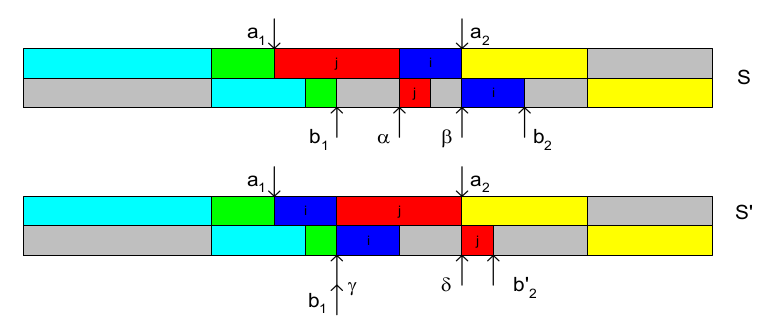
\includegraphics[scale=0.5]{zad7}
$S^\prime$ - $S$ z zamienionymi zadaniami $i,j$\\
$b_{1}$ - zakończenie poprzedniego (przed $i$) zadania w $S$\\
$b_{1}^\prime$ - zakończenie poprzedniego (przed $j$) zadania w $S^\prime$\\
$b_{2}$ - zakończenie obu zadań w $S$\\
$b_{2}^\prime$ - zakończenie obu zadań w $S^\prime$\\\\
$\alpha = \max(b_1, (A_j + a_1))$ rozpoczęcie pierwszego zadania $b$ w $S$\\
$\beta = \max(a_2, (B_j + \alpha))$ rozpoczęcie drugiego zadania $b$ w $S$\\
$b_2 = B_i + \beta = \max(a_1+A_j+A_i+B_i, B_j + B_i +b_1, B_j+B_i +A_j+a_1)$\\
$\gamma = \max(b_1,(A_i+a_1))$ rozpoczęcie pierwszego zadania $b$ w $S^\prime$\\
$\delta = \max(a_2,(B_i+\gamma))$ rozpoczęcie drugiego zadania $b$ w $S^\prime$\\
$b_2^\prime = B_j + \delta = \max(a_1+A_j+A_i+B_j, B_j + B_i +b_1, B_j+B_i +A_i+a_1)$\\
\clearpage
\begin{enumerate}
    \item $j \in S_2 \land i \in S_1 \implies A_j \geq B_j \land A_i < B_i$:
    $$
    \overbrace{a_1 + A_j + A_i + B_i}^{1. \quad w \quad b_2} \geq \underbrace{B_i + B_j + A_i + a_1}_{3. \quad w \quad b_2^\prime}
    $$
    $$
    \overbrace{B_j + B_i + A_j + a_1}^{3. \quad w \quad b_2} \geq \underbrace{a_1 + A_j + A_i + B_j}_{1. \quad w \quad b_2^\prime}
    $$
    \item $i,j \in S_1 \land A_j > A_i \implies A_j > A_i \land A_i < B_i$
    $$
    \overbrace{B_j + B_i + A_j + a_1}^{3. \quad w \quad b_2} > \underbrace{B_i + B_j + A_i + a_1}_{3. \quad w \quad b_2^\prime}
    $$
    $$
    \overbrace{B_j + B_i + A_j + a_1}^{3. \quad w \quad b_2} > \underbrace{a_1 + A_j + A_i + B_j}_{1. \quad w \quad b_2^\prime}
    $$
    \item $i,j \in S_2 \land B_j < B_i \implies A_j \geq B_j \land B_j < B_i$
    $$
    \overbrace{a_1 + A_j + A_i + B_i}^{1. \quad w \quad b_2} \geq \underbrace{B_i + B_j + A_i + a_1}_{3. \quad w \quad b_2^\prime}
    $$
    $$
    \overbrace{a_1 + A_j + A_i + B_i}^{1. \quad w \quad b_2} > \underbrace{a_1 + A_j + A_i + B_j}_{1. \quad w \quad b_2^\prime}
    $$
\end{enumerate}
W każdym przypadku mamy: $b_2 \geq b_2^\prime$. Zmiana nie pogarsza rozwiązania.
\end{proof}
\href{https://personal.utdallas.edu/~chandra/documents/6363/lec7.pdf}{źródło}
\clearpage
\setcounter{lemma}{0}
\section{Zadanie 8}
\begin{lemma}
Jeżeli strategi zachłanna nie zwraca OPT'a to najmniejszy kontrprzykład $x$ jest w przedziale:
$$
b + 1 < x < a + b
$$
\end{lemma}
\begin{proof}
\subsection*{\\$b+1 < x$}
Rozważmy przypadki:
\begin{enumerate}
    \item $x < b$ \quad\quad\quad\quad dobieramy jak OPT, same $a$ z $1$ lub same $1$.
    \item $x = b \quad(+ 1)\quad $ dobieramy jak OPT, tylko $b$ (z $1$)
\end{enumerate}
\subsection*{\\$x < a + b$}
Weźmy dowolny $x \geq a + b$ i załóżmy, że $\forall_{y < x}OPT(y) = GRD(y)$:
\begin{enumerate}
    \item $b$ jest w OPT \quad $OPT(x) = OPT(x-b) + 1 = GRD(x-b) + 1 = GRD(x)$
    \item $a$ jest w OPT \quad \begin{align*}GRD(x) = GRD(x-b)+1 =  OPT(x-b) + 1 \leq OPT(x-b-a) + 2 &=\\ GRD(x-b-a) +2  = GRD(x-a) + 1  = GRD(x)\end{align*}
    \item $1$ jest w OPT \quad \begin{align*}GRD(x) = GRD(x-b) +1 =OPT(x-b) + 1 \leq OPT(x-b-1) + 2 &=\\ GRD(x-b-1) +2  = GRD(x-1) + 1  = OPT(x-1) + 1 = OPT(x) \leq GRD(x)\end{align*}
\end{enumerate}
Z dowolności wyboru $x$ pokazaliśmy, że jeżeli istnieje kontrprzykład to musi też istnieć kontrprzykład $< a+b$
\end{proof}
\clearpage
\begin{theorem}
Strategia zachłanna z nominałami $\{1,a,b\}$ nie zwraca OPT'a wtedy i tylko wtedy gdy:
$$
0 < r < a - q
$$
gdzie: $b = qa + r$ oraz $r \in [0,a-1]$
\end{theorem}
\begin{proof}
\subsection*{\\$(\implies)$}
Niech $x$ będzie najmniejszym kontrprzykładem (zakładamy, że zachłan nie zwraca OPT'a). Z lematu 1. wiemy, że $x \in [b+2, a+b-1]$. BSO (z dokładnością do jedynek, gdzie różnią się rozwiązania) GRD = $(e,0,1)$ OPT = $(0,k,0)$ \\oczywiście $e \in [2, a-1]$, dalej przyrównujemy rozkłady $x$:
$$
x = b + e = k\cdot a
$$
$$
b = k\cdot a - e = \underbrace{(k-1)}_q\cdot a + \underbrace{(a-e)}_r
$$
z powyższych rozważan:
$$
r = a - e \geq a - (a-1) =1 > 0
$$
założyliśmy, że zachłan zwraca gorszy wynik więc $\underbrace{e + 1}_{GRD} > \overbrace{k}_{OPT} \implies e > k-1$:
$$
a - q = a - (k-1) > a - e = r
$$


\subsection*{\\$(\impliedby)$}
Rozważmy $x=a+b-1$, zachłan zwróci $(a-1,0,1)$, ale $$x = a + \underbrace{qa + r}_b - 1 =(q+1)\cdot a + (r-1)$$ czyli $x = (r-1,q+1,0)$, stąd OPT $\leq r-1 + q+1 = r+q$\\Z założenia:
$$
0 < r < a - q \implies r + q < a
$$
wobec powyższego, zachłan zwróci rozwiązanie gorsze od OPT'a:
$$
OPT \leq r + q < a = a - 1 + 1 = GRD
$$
\end{proof}
\begin{python}
r = b%a
q = (b-r)/a
return not (0 < r and r < a-q)
\end{python}
\clearpage
\setcounter{lemma}{0}
\section{Zadanie 9}
\begin{python}
q = priority_queue() # minimow
for w in W:
    q.push(Node(w,(NULL,NULL)))
while q.size() >= 2:
    u = q.pop()
    v = q.pop()
    q.push(Node(u.w+v.w,(u,v))) # (waga,(dzieci))
return q.pop() # root
\end{python}
\begin{lemma}
Niech $w,w^\prime$ najmniejsze wagi z $\{w_1,\ldots,w_n\}$. Istnieje optymalne drzewo $T$ tż. liście o wagach $w,w^\prime$, mają wspólnego rodzica.
\end{lemma}
\begin{proof}
Oczywiście wierzchołek o maksymalnej głębokości ma \textit{brata} w OPT $T$, w przeciwnym przypadku możemy go \textit{przechnąć} w górę i tym zmniejszymy zewnętrzną długość drzewa.\\
Rozważmy drzewo $T^\prime$, z zamienionymi maksymalnie głębokimi $u,v$ liśćmi z minimalnymi wagami $V_{w}, V_{w^\prime}$.\\
\begin{align*}
EL(T) - EL(T^\prime) \geq c(V_w)d_T(V_w) + c(u)d_T(u) - c(V_w)d_T(u) - c(u)d_T(V_w) =\\
 c(V_{w})\cdot (d_T(V_w) - d_T(u)) + c(u)\cdot (d_T(u) - d_T(V_w)) = \\ \underbrace{(c(u) - c(V_w))}_{\geq 0} \cdot \underbrace{(d_T(u) - d_T(V_w))}_{\geq 0} \geq 0
\end{align*}
Analogicznie dla drugiej pary zmienianych ze sobą wierzchołków $v,V_{w^\prime}$
\end{proof}
\begin{proof}
\clearpage
\subsection*{Poprawność}
\subsection*{Baza}
Dla $n \in \{1,2\}$ OK
\subsection*{Krok}
Załóżmy, że dla $n$ algorytm zwraca optymalne drzewo $T$. Dla $n+1$:\\
$w,w^\prime$, najmniejsze wagi z $W$, $|W| = n+1$, $W^\prime = W \setminus\{w,w^\prime\} \cup \{w+w^\prime\}$\\\\
$P$ - drzewo zwrócone przez algorytm dla danych wejściowych $W$\\
$P^\prime$ - drzewo zwrócone przez algorytm dla danych wejściowych $W^\prime$ (z założenia indukcyjnego, $P^\prime$ = OPT)\\
Pokażemy, że $P$ też jest optymalne:\\\\
Oznaczmy $T$ jako drzewo optymalne dla wejścia $W$, z lematu 1. BSO zakładamy, że $V_w,V_{w^\prime}$ są najniższymi liśćmi i \textit{braćmi}. Usuńmy zatem $V_w,V_{w^\prime}$ z $T$ i za wagę ich ojca ustawmy $w+w^\prime$. Otrzymamy drzewo $T^\prime$ z wagami liści równymi zbiorowi $W^\prime$. Oczywiście $EL(T^\prime) \geq EL(P^\prime)$ ($P^\prime$ to OPT).\\
Pamiętamy jeszcze $d(V_w) = d(V_{w^\prime})$ bo to \textit{bracia}, zatem:
$$
EL(T) = EL(T^\prime) - (d(V_w)-1)(c(V_w) + c(V_{w^\prime})) + d(V_w)(c(V_w) + c(V_{w^\prime}))
$$
$$
EL(P) = EL(P^\prime) - (d(V_w)-1)(c(V_w) + c(V_{w^\prime})) + d(V_w)(c(V_w) + c(V_{w^\prime}))
$$
Dalej:
$$
EL(T^\prime) - EL(T) = EL(P^\prime) - EL(P)
$$
$$
EL(T^\prime) -EL(P^\prime) = EL(T) - EL(P)
$$
wnioskujemy:
$$
EL(T) \geq EL(P)
$$
Stąd $P$ - OPT bo $T$ było OPT'em.
\end{proof}
\end{document}

